%%%%%%%%%%%%%%%%%%%%%%%%%%%%%%%%%%%%%%%%%
% Beamer Presentation
% LaTeX Template
% Version 1.0 (10/11/12)
%
% This template has been downloaded from:
% http://www.LaTeXTemplates.com
%
% License:
% CC BY-NC-SA 3.0 (http://creativecommons.org/licenses/by-nc-sa/3.0/)
%
%%%%%%%%%%%%%%%%%%%%%%%%%%%%%%%%%%%%%%%%%

%----------------------------------------------------------------------------------------
%	PACKAGES AND THEMES
%----------------------------------------------------------------------------------------

\documentclass{beamer}
\usepackage[spanish]{babel}
\usepackage{subcaption}
\usepackage{hyperref}
\usepackage{amssymb, amsmath}
\usepackage{amsthm}
\usepackage{soul}
\usepackage{booktabs}
\usepackage{graphicx}
\usepackage{epigraph}
\usepackage{enumitem}
\usepackage{xcolor}

\usepackage{stackengine}

\usepackage{algorithm,algorithmic}

% Configuración básica del tema
\mode<presentation> {

% The Beamer class comes with a number of default slide themes
% which change the colors and layouts of slides. Below this is a list
% of all the themes, uncomment each in turn to see what they look like.

%\usetheme{default}
%\usetheme{AnnArbor}
%\usetheme{Antibes}
%\usetheme{Bergen}
%\usetheme{Berkeley}
%\usetheme{Berlin}
%\usetheme{Boadilla}
%\usetheme{CambridgeUS}
%\usetheme{Copenhagen}
%\usetheme{Darmstadt}
%\usetheme{Dresden}
%\usetheme{Frankfurt}
%\usetheme{Goettingen}
%\usetheme{Hannover}
%\usetheme{Ilmenau}
%\usetheme{JuanLesPins}
%\usetheme{Luebeck}
%\usetheme{Madrid}
%\usetheme{Malmoe}
%\usetheme{Marburg}
%\usetheme{Montpellier}
%\usetheme{PaloAlto}
%\usetheme{Pittsburgh}
%\usetheme{Rochester}
%\usetheme{Singapore}
%\usetheme{Szeged}
%\usetheme{Warsaw}
\usetheme{metropolis}   
\newcommand\myeq{\stackrel{\mathclap{\normalfont\mbox{?}}}{\subsetneq}}
% As well as themes, the Beamer class has a number of color themes
% for any slide theme. Uncomment each of these in turn to see how it
% changes the colors of your current slide theme.


%\setbeamertemplate{footline} % To remove the footer line in all slides uncomment this line
\setbeamertemplate{footline}[page number] % To replace the footer line in all slides with a simple slide count uncomment this line

\setbeamertemplate{navigation symbols}{} % To remove the navigation symbols from the bottom of all slides uncomment this line
}

\usepackage{graphicx} % Allows including images
\usepackage{booktabs} % Allows the use of \toprule, \midrule and \bottomrule in tables


%----------------------------------------------------------------------------------------
%	TITLE PAGE
%----------------------------------------------------------------------------------------

\title[Short title]{My favorite proof method}
\subtitle{Lightning talk}

\author{Presented by: \\Pedro Bonilla Nadal (pedrobn@)\\[0.25cm]\\\medskip} % Your name




\institute[Universidad de Granada]{
\\ % Your institution for the title page
\medskip
}



\begin{document}

                     
\begin{frame}

  \titlepage % Print the title page as the first slide

\end{frame}

\begin{frame}{Overview}
\tableofcontents
\end{frame}

% %----------------------------------------------------------------------------------------
% %	PRESENTATION SLIDES
% %----------------------------------------------------------------------------------------

% %------------------------------------------------

\section{Existence by probability}
\begin{frame}{A new proof method}
 The probabilistic method is a useful method to prove the existence of objects
 with an specific property.
  \begin{enumerate}
  \item Define the space.
  \item Define how to generate objects.
  \item Check the probability on a random object.
  \item Profit. 
  \end{enumerate}
\end{frame}

\begin{frame}
 \begin{itemize}
\item Philosophy: instead of giving the object explicitly, we consider a random object and compute the probability of satisfying the property. 
\item Great for decision problems.
\item Many of its examples are thanks to Paul Erd\H{o}s.
\end{itemize}
\end{frame}

\section{Some theorems}
% \begin{frame}{An useful tool}
% \begin{theorem}[Lovász Local Lema]\label{LLL}
% 	Let $\Omega$ be a probability space and let 
% $\mathcal{A} = \{A_1,...,A_m\}$ be arbitrary events in this space. Let $G$ be a lopsidependency graph for $\mathcal{A}$. If there exists a mapping $\mu:\mathcal{A} \to (0,1)$ such that 
% $$
% \forall A \in \mathcal{A} : P (A) \le \mu(A) \prod_{B\in\Gamma_G(A)} (1-\mu(B)),
% $$

% then $P\left ( \bigcap_{A\in \mathcal{A}} \overline{A}\right ) > 0$.\\
% \end{theorem}
 
% \end{frame}
\begin{frame}{SAT problem}
  Given a propositional logic formula, check out whether it exists a truth assignment that satisfy the formula.
  \begin{example}   
    \begin{itemize}
    \item $(x\lor y)\land (\neg y \lor  \neg x)$ is satisfiable by $x\to \top, y \to \bot$.
    \item    $(\neg x \lor y)\land (z\lor \neg y) \land (\neg z ) \land (x)$ is not satisfiable.
  \end{itemize}
\end{example}

Usually formulas are presented as disjoints of clauses (also called conjunctions), as in the example. Therefore the problem is to solve every clause at the same time. Original NP-complete problem.\\
Finally, $\Gamma^*_G(A)$ is the graph with vertex the clauses of a formula $G$, and there is an edge between $C$ and $D$ iff they conflict in some variable.
\end{frame}

\begin{frame}{Lovasz Local Lemma}


\begin{theorem}[Lovász Local Lemma for SAT]\label{LLLS}
  Let $F = C_1\land ... \land C_n$ be a formula. If there exists a mapping $\mu:\{C_1,...,C_n\}\to (0,1)$ that associates a number with each clause in the formula. We define the event:
  $$A_i = \left[C_i\text{ \stackanchor{ being falsified by a random}{  truth assignment}}\right],$$
	If it happens
	$$
\forall i \in 1,..,,n : P () \le \mu() \prod_{D\in\Gamma^*_G(C)} (1-\mu(D)),
$$
	then the $P(\cap_{i=1}^n \neg A_i)$ F is satisfiable.
\end{theorem}
\end{frame}

\begin{frame}{Corollary}
\begin{corollary}
	Let $F$ be a formula on which each clause have $k$ variables. If  $\ \forall C \in F$ and $\ |\Gamma_F(C)|\le 2^k/e-1$ then $F$ is satisfiable.
      \end{corollary}
      
\end{frame}
\section{Constructivist approach}
\begin{frame}{The revenge of the contructivist I}
Moser proves that there exists an algorithm such that it gives an assignment satisfying the SAT formula, should it happen that the formula satisfies \ref{LLLS} conditions. This is no a big deal, as a backtrack would be also capable of providing the solution, given that we know its existence. Not so trivial is that it would run in $O(|F|)$. 
\end{frame}


\begin{frame}{The revenge of the contructivist II}
\begin{figure}[h]
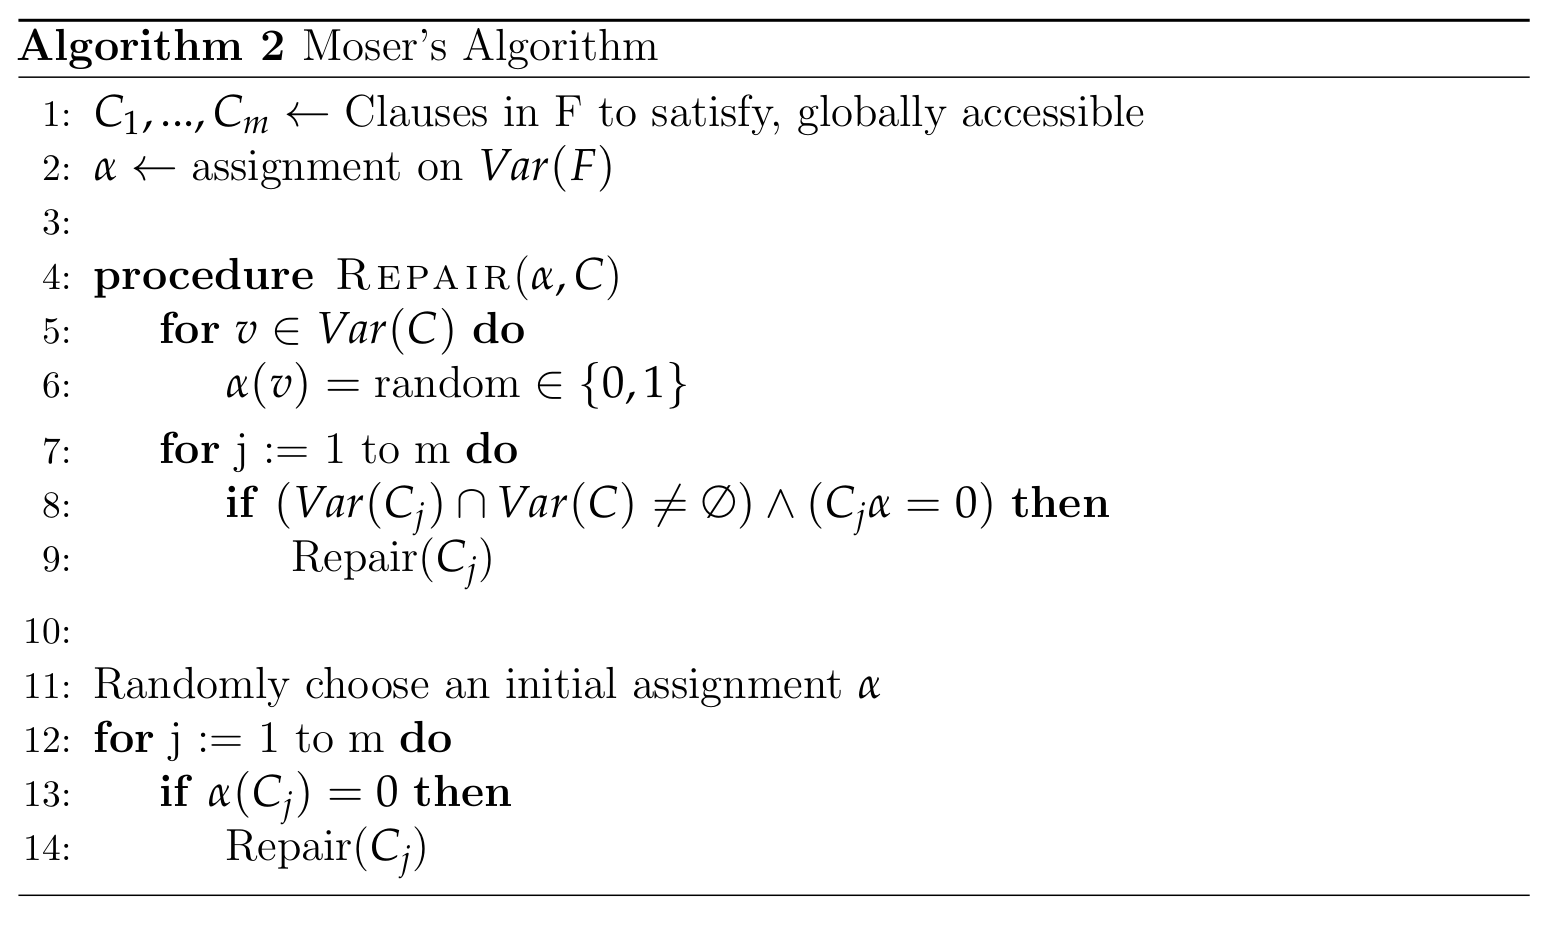
\includegraphics[width=0.8\textwidth]{screenshot.png}
\end{figure}
\end{frame}



% \section{Bibliografía}
% \begin{thebibliography}{9}


% \begin{frame}{Bibliography}


% \bibitem{intro}
% Moser, Robin. \textit{Exact Algorithms for Constraint Satisfaction Problems}. Logos Verlag Berlin GmbH, 2013.





% \end{frame}{}

% \end{thebibliography}

\begin{frame}[standout]
  Thanks for coming.
\end{frame}
\end{document}

